\begin{apendicesenv}

\partapendices

\chapter{Histórias de usuário}
\label{apen-historia-usuario}
% história
\begin{description}

% ---------------------------------------------------------------------
\item [US01\label{us01}] \underline{Definir tempo restante}

\textbf{Como} um professor

\textbf{Gostaria de} definir o tempo restante para cada atividade no Work Assignment

\textbf{Para} gerenciar o envio de atividades pelos alunos em um determinado período.

\subsubsection*{Cenários de uso:}

\begin{enumerate}
\item \underline{Definir tempo}

\textbf{[Dado]} que esteja logado como professor

\textbf{[E]} selecione a o opção ``Gerenciar conteúdo''

\textbf{[Quando]} eu clicar em trabalho a ser entregue

\textbf{[Então]} devo visualizar a opção ``Ativar tempo de entrega''

\textbf{[E]} informar a data e hora máxima para envio da atividade.

\item \underline{Modificar tempo}

\textbf{[Dado]} que esteja logado como professor

\textbf{[E]} eu tenha atividades a ser entregue em aberto

\textbf{[E]} eu esteja visualizando as informações da atividade

\textbf{[Quando]} eu selecionar opção ``Editar''

\textbf{[E]} visualizar a opção ``Tempo de entrega''

\textbf{[Então]} deve ser permitido que eu altere o tempo definido

\textbf{[E]} visualize o resultado da alteração após a confirmação.

\item \underline{Permitir entrega de atividades após período}

\textbf{[Dado]} que esteja logado como professor

\textbf{[E]} selecione a o opção ``Gerenciar conteúdo''

\textbf{[E]} vavegar até a página trabalho a ser entregue

\textbf{[Quando]} selecionar a opção ``Ativar tempo de entrega''

\textbf{[Então]} devo visualizar a opção ``Permitir entrega após o período''

\textbf{[Para]} que eu possa selecioná-la.

\end{enumerate}

% -----------------------------------------------------------------------
\item [US02\label{us02}]\underline{Visualizar tempo restante de atividades}

\textbf{Como} um aluno

\textbf{Gostaria de} visualizar o tempo restante da atividade

\textbf{Para} enviar um arquivo na data correta.

\subsubsection*{Cenários de uso:}

\begin{enumerate}
\item \underline{Visualizar tempo}

\textbf{[Dado]} que esteja logado como Aluno

\textbf{[E]} eu esteja inscrito em um Curso

\textbf{[E possua atividade em aberto]}

\textbf{[Quando]} eu selecionar a opção de visualizar a atividade

\textbf{[Então]} eu devo visualizar se a atividade está em aberto

\textbf{[E]} qual o tempo restante para o envio da atividade.

\end{enumerate}

% -----------------------------------------------------------------------

\item [US03\label{us03}] \underline{Atribuir notas aos alunos}

\textbf{Como} um professor

\textbf{Gostaria de} atribuir notas as atividades enviadas pelos alunos

\textbf{Para} avaliar o rendimento de cada um deles.

\subsubsection*{Cenários de uso:}

\begin{enumerate}
\item \underline{Atribuir notas}

\textbf{[Dado]} que esteja logado como professor

\textbf{[E]} que a funcionalidade de notas esteja habilitada no plugin

\textbf{[Quando]} selecionar uma atividade na lista de atividades

\textbf{[Então]} devo visualizar a opção atribuir nota

\textbf{[E]} devo visualizar o campo ``nota'' para preenche-lo.


\item \underline{Alterar notas}

\textbf{[Dado]} que esteja logado como professor

\textbf{[E]} que a funcionalidade de notas esteja habilitada no plugin

\textbf{[Quando]} selecionar uma atividade na lista de atividades

\textbf{[E]} atividade já possua notas

\textbf{[Então]} devo visualizar a opção alterar nota

\textbf{[E]} devo visualizar o campo ``nota'' para preenche-lo.

\item \underline{Definir critério da nota final}

\textbf{[Dado]} que esteja logado como professor

\textbf{[E]} que a funcionalidade de notas esteja habilitada no plugin

\textbf{[Quando]} criar um trabalho a ser enviado

\textbf{[Então]} devo visualizar a opção de qual o critério para nota final

\textbf{[E]} devo selecionar qual a opção desejada.

\end{enumerate}

% -----------------------------------------------------------------------

\item [US04\label{us04}] \underline{Publicar notas aos alunos}

\textbf{Como} um professor

\textbf{Gostaria de} publicar as notas atribuídas as atividades

\textbf{Para} que os alunos possam visualizar suas respectivas avalizações

\subsubsection*{Cenários de uso:}

\begin{enumerate}
\item \underline{Disponibilizar notas de uma determinada atividade}

\textbf{[Dado]} que esteja logado como professor

\textbf{[E]} que a funcionalidade de notas esteja habilitada no plugin

\textbf{[Quando]} selecionar uma atividade na lista de atividades

\textbf{[Então]} devo visualizar a opção ``permitir visualização''

\textbf{[E]} devo ter a opção de ativá-lo.

\item \underline{Omitir notas de uma determinada atividade}

\textbf{[Dado]} que esteja logado como professor

\textbf{[E]} que a funcionalidade de notas esteja habilitada no plugin

\textbf{[Quando]} selecionar uma atividade na lista de atividades

\textbf{[Então]} devo visualizar a opção ``permitir visualização''

\textbf{[E]} devo ter a opção de desativá-lo.

\end{enumerate}

% -----------------------------------------------------------------------
\item [US05\label{us05}]\underline{Visualização das notas}

\textbf{Como} um aluno

\textbf{Gostaria de} visualizar minhas notas

\textbf{Para} inteira-me sobre minha pontuação nas atividades.

\subsubsection*{Cenários de uso:}
\begin{enumerate}

\item \underline{Visualizar cursos com notas disponíveis}

\textbf{[Dado]} que estou logado como ``Hebert''

\textbf{[E]} o plugin Work Assignment esteja ativo

\textbf{[E]} participo de alguma comunidade que utilize o plugin de notas

\textbf{[E]} existem notas de atividades disponíveis

\textbf{[E]} o professor tenha permitido sua visualização

\textbf{[Quando]} eu navegar até a página ``Minhas notas''

\textbf{[Então]} tenho que ver todos as comunidades (cursos) com notas disponíveis.

\item \underline{Detalhar notas de cada curso}

\textbf{[Dado]} que estou logado como ``Hebert''

\textbf{[E]} o plugin Work Assignment esteja ativo

\textbf{[E]} participo de alguma comunidade que utilize o plugin de notas

\textbf{[E]} existem notas de atividades disponíveis

\textbf{[E]} o professor tenha permitido sua visualização

\textbf{[E]} navegar até a página ``Minhas notas''

\textbf{[E]} visualizar todos as comunidades (cursos) com notas disponíveis

\textbf{[Quando]} eu selecionar a ``Visualizar detalhes'' de alguma comunidade

\textbf{[Então]} tenho que ver todos os grupos de atividades

\textbf{[E]} as notas disponibilizadas pelo professor.

\end{enumerate}

% -----------------------------------------------------------------------
\item [US06\label{us06}]\underline{Professor gerencia notas}

\textbf{Como} um professor

\textbf{Gostaria de} gerenciar as notas dos integrantes da comunidade

\textbf{Para} manter o controle sobre a pontuação de todos os alunos.

\subsubsection*{Cenários de uso:}

\begin{enumerate}

\item \underline{Definir grupo de atividades}

\textbf{[Dado]} que esteja logado como professor

\textbf{[E]} que a funcionalidade de notas esteja habilitada no plugin

\textbf{[E]} selecionar a opção ``Gerenciar notas''

\textbf{[E]} e eu selecionar o curso desejado

\textbf{[Quando]} eu clicar em ``Cadastrar grupo de atividades''

\textbf{[E]} eu preencho os campos \\
``Nome do grupo'',\\
e ``Lista de Atividades''\\
\textbf{[E]} eu clico em ``Salvar''

\textbf{[Então]} recebo uma mensagem de confirmação

\textbf{[E]} visualizo todas os grupos de atividades criados.

\item \underline{Visualizar notas de todos os alunos de uma determinada atividade}

\textbf{[Dado]} que esteja logado como professor

\textbf{[E]} que a funcionalidade de notas esteja habilitada no plugin

\textbf{[E]} selecionar a opção ``Gerenciar notas''

\textbf{[E]} e eu selecionar o curso desejado

\textbf{[Quando]} eu selecionar atividade

\textbf{[E]} algum aluno tenha enviado a atividade

\textbf{[Então]} devo visualizar todas as atvidades enviadas e suas respectivas notas.

\item \underline{Visualizar notas de todos ao alunos de um grupo de atividades}

\textbf{[Dado]} que esteja logado como professor

\textbf{[E]} que a funcionalidade de notas eteja habilitada no plugin

\textbf{[E]} selecionar a opção ``Gerenciar notas''

\textbf{[E]} e eu selecionar o curso desejado

\textbf{[Quando]} eu clicar em ``Visualizar notas por grupo de atividades''

\textbf{[E]} algum aluno tenha enviado a atividade

\textbf{[Então]} devo visualizar todas as atvidades daquele grupo e suas respectivas notas.

\end{enumerate}

% -----------------------------------------------------------------------

\item [US07\label{us07}] \underline{Bloco de notas recentes}

\textbf{Como} um aluno

\textbf{Gostaria de} visualizar minhas cinco últimas notas

\textbf{Para} facilitar a visualização do meu desempenho no curso.

\subsubsection*{Cenários de uso:}

\begin{enumerate}

\item \underline{Adicionar bloco}

\textbf{[Dado]} que esteja logado como aluno

\textbf{[Quando]} eu navegar até meu painel de controle

\textbf{[E]} eu selecionar a opção ``Editar Blocos Laterais''

\textbf{[E]} eu clicar na opção ``Adicionar bloco''

\textbf{[Então]} devo visualizar a opção ``Notas Recentes''

\textbf{[E]} devo ter a opção de adicioná-lo.

\item \underline{Visualizar cinco notas recentes}

\textbf{[Dado]} que esteja logado como aluno

\textbf{[E]} esteja com o bloco de notas recentes adicionado

\textbf{[E]} o professor tenha publicado alguma nota

\textbf{[Então]} devo visualizar o bloco com minhas cinco últimas notas

\textbf{[E]} o nome de cada atividade.

\end{enumerate}

% -----------------------------------------------------------------------

\item [US08\label{us08}] \underline{Bloco para visualização dos módulos}

\textbf{Como} um professor

\textbf{Gostaria de} visualizar um bloco com todos os módulos disponíveis no meu curso

\textbf{Para} facilitar a visualização da organização do curso criado.

\subsubsection*{Cenários de uso:}

\begin{enumerate}

\item \underline{Adicionar bloco}

\textbf{[Dado]} que esteja logado como professor

\textbf{[E]} e seja administrador da comunidade

\textbf{[Quando]} eu navegar até painel de controle da comunidade

\textbf{[E]} eu selecionar a opção ``Editar Blocos Laterais''

\textbf{[E]} eu clicar na opção ``Adicionar bloco''

\textbf{[Então]} devo visualizar a opção ``Lista de Grupos de trabalhos a serem enviados''

\textbf{[E]} devo ter a opção de adicioná-lo.

\item \underline{Editar numero de atividades listadas no bloco}

\textbf{[Dado]} que esteja logado como professor

\textbf{[E]} e seja administrador da comunidade

\textbf{[Quando]} eu navegar até painel de controle da comunidade

\textbf{[E]} eu selecionar a opção ``Editar Blocos Laterais''

\textbf{[E]} eu clicar na opção ``Editar bloco''

\textbf{[Então]} devo visualizar a opção ``Limite de trabalhos enviados''

\textbf{[E]} permitir escolher o número de itens a serem visualizados.

\item \underline{Visualizar módulos}

\textbf{[Dado]} que esteja logado como aluno

\textbf{[E]} seja membro da comunidade

\textbf{[E]} a comunidade possua grupos de atividades a serem enviadas

\textbf{[E]} possua trabalhos a serem enviados

\textbf{[Então]} devo visualizar o bloco todos os módulos disponíveis

\textbf{[E]} as atividades relacionadas a cada um deles.

\end{enumerate}

\item [US09\label{us09}]\underline{Autenticação via LDAP}

\textbf{Como} um aluno da Universidade Brasília

\textbf{Gostaria de} me autenticar na rede através da minha matrícula e senha

\textbf{Para} utilizar os mesmos dados de cadastro da UnB.

\subsubsection*{Cenários de uso:}

% cenário
\begin{enumerate}
\item \underline{Acesso sem matrícula cadastrada}

\textbf{[Dado]} que sou aluno da UnB

\textbf{[E]} possuo cadastro ativo na base de dados da UnB

\textbf{[E]} possuo cadastro ativo na base de dados do Comunidade.UnB

\textbf{[Quando]} eu acessar o portal

\textbf{Como} um aluno da Universidade Brasília

\textbf{[Então]} devo ser direcionado para uma página com o título ``Cadastrar Matrícula''

\textbf{[E]} devo ver os campos ``Matrícula'', ``Senha'' e
``confirmação de senha'' em branco.

\item \underline{Registro de matrícula de usuários existentes}

\textbf{[Dado]} que sou aluno da UnB

\textbf{[E]} me encontro na página de Cadastrar matrícula do Comunidade.UnB

\textbf{[Quando]} eu preencher os campos \\
``matrícula'' com ``100103979'',\\
e ``senha''  com a senha da base dados da UnB,\\
e ``confirmação de senha''

\textbf{[E]} clicar no botão ``Registrar''

\textbf{[Então]} eu devo ser direcionado para meu perfil
% cenários
\end{enumerate}

% historia
\end{description}

\chapter{Instruções para preenchimento do questionário}
\label{apen-inst}
Caros,

O estudo a seguir faz parte de uma pesquisa realizada por um aluno de Engenharia de \emph{software}, da Universidade de Brasília – \textbf{UnB}, o qual será utilizado como forma de obtenção de conhecimento sobre o tema.

Esta pesquisa visa investigar se os alunos da Universidade de Brasília utilizam as redes sociais, como o \textit{Facebook}, para o compartilhamento de recursos e informações relacionados as disciplinas cursadas na Universidade. Para tanto, necessito de sua colaboração respondendo ao questionário sobre o tema. É importante ressaltar que os dados aqui levantados serão compilados e utilizados apenas para fins acadêmicos, na problematização da pesquisa.

Instruções para preenchimento do questionário:
\begin{enumerate}
\item Você deverá selecionar um item para indicar o grau de concordância com as assertivas apresentadas na tabela \ref{tab:preenchimento}.

\begin{table}[h]
\center
\begin{tabular}{|c|c|c|c|c|}
\hline
		\textbf{NUNCA} & \textbf{RARAMENTE} & \textbf{ÀS VEZES} & \textbf{FREQUENTEMENTE} & \textbf{SEMPRE}\\ \hline
\end{tabular}
\caption{Opções para preenchimento do questionário.}
\label{tab:preenchimento}
\end{table}
\textbf{Lembrando} que quanto mais próximo de \textbf{Nunca}, \textbf{MENOR} o grau de concordância. Quanto mais próximo de \textbf{Sempre}, \textbf{MAIOR} o grau de concordância.

\item O questionário deve ser respondido pelos alunos das Universidade de Brasília;

\item Não existem respostas ``certas'' ou ``erradas''. O importante é respondê-las de forma \textbf{sincera}.

\item Procure não deixar nenhuma resposta em branco. Sua participação é muito importante para a finalização deste trabalho.
\end{enumerate}

Desde já agradeço sua atenção e cooperação. Coloco-me à disposição para os esclarecimentos que se fizerem necessários.

Cordialmente,
\begin{description}
\item Hebert Douglas de Almeida Santos <hebertdougl@gmail.com>
\end{description}

\chapter{Questionário para problematização}
\label{apen-quest}

\begin{enumerate}
% \item \label{itm-first} Você utiliza algum tipo de rede social para uso pessoal?

\item \label{pergunta1} Com que frequência você utiliza redes sociais?

\item \label{pergunta2} Você utiliza alguma rede social como ferramenta de apoio as disciplinas?

\item \label{pergunta3} Os professores incentivam o uso de redes sociais para suas disciplinas?

\item \label{pergunta4} Mesmo que o professor não recomende o uso de redes sociais para discussão de conteúdos de suas disciplinas, você as utiliza?

\end{enumerate}


\chapter{Avaliação dos resultados}
\label{apen-quest-result}

\begin{figure}[h]
    \centering
    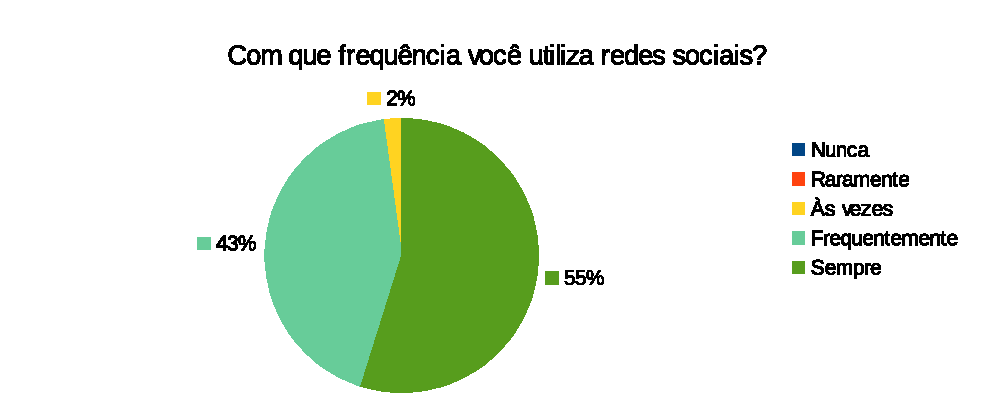
\includegraphics[keepaspectratio=true,scale=1]
      {figuras/pergunta1p.eps}
    \caption{Resultados do questionário para a pergunta \ref{pergunta1}}
    \label{pergunta1}
\end{figure}

\begin{figure}[h]
    \centering
    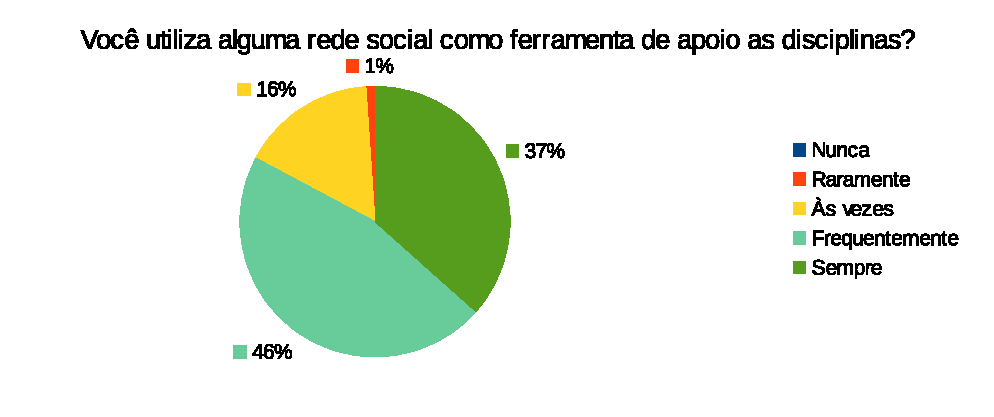
\includegraphics[keepaspectratio=true,scale=1]
      {figuras/pergunta2p.eps}
    \caption{Resultados do questionário para a pergunta \ref{pergunta2}}
    \label{pergunta2}
\end{figure}

\begin{figure}[h]
    \centering
    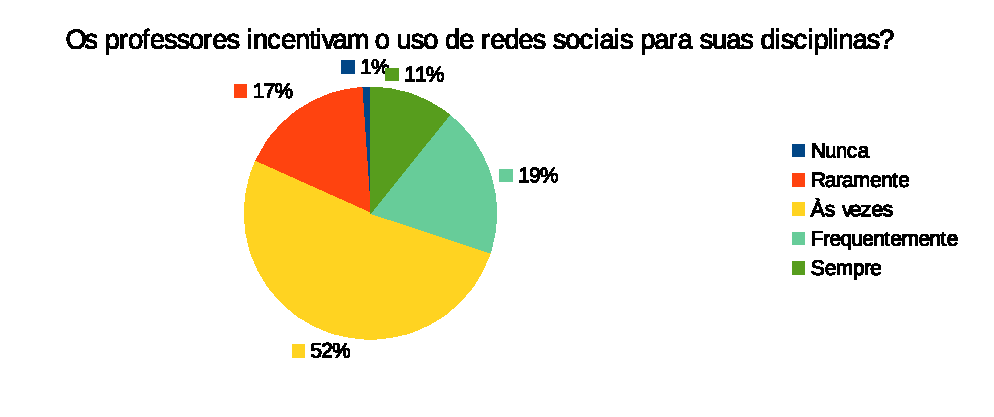
\includegraphics[keepaspectratio=true,scale=1]
      {figuras/pergunta3p.eps}
    \caption{Resultados do questionário para a pergunta \ref{pergunta3}}
    \label{pergunta3}
\end{figure}

\begin{figure}[h]
    \centering
    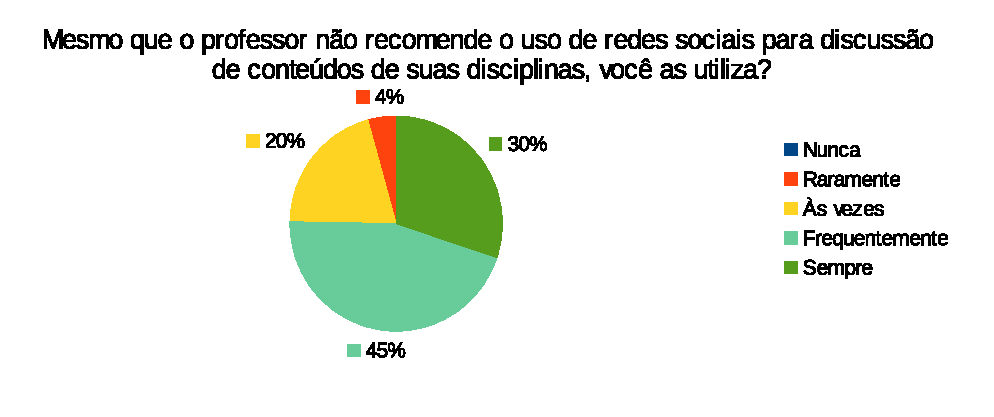
\includegraphics[keepaspectratio=true,scale=1]
      {figuras/pergunta4p.eps}
    \caption{Resultados do questionário para a pergunta \ref{pergunta4}}
    \label{pergunta4}
\end{figure}

\end{apendicesenv}